\section{Comparison of EAToF and EDXRD}
\subsection{EAToF results}
Four Duracell MN1500 AA alkaline cells were discharged at 143, 200, 300 and 400 mA while performing EAToF measurements. The discharge capacity at each rate is shown in Table~\ref{tab:captable}.

\begin{table}[htb]
\centering
  \caption{\label{tab:captable}Alkaline AA battery discharge capacity at multiple discharge rates.}
  \begin{tabular}[t]{*{2}{l}}
    \hline
       Discharge rate (mA) & \specialcell{Capacity (mAh)}\\
    \hline
        143 & 2496\\
        200 & 2264\\
        300 & 2012\\
        400 & 1734\\
  \end{tabular}
\end{table}

To show the time-evolution of the individual acoustic waveforms, we composited all measurements for each cell into a two-dimensional intensity map, plotting cycle time against ToF data. This allowed for ready visualization of the relative intensity of the ultrasonic signal as well as the shifts in ToF that occur during discharge. Figure~\ref{fig:alkbwrates} shows the resulting time-resolved transmitted acoustic signal intensity maps, the normalized total transmitted signal amplitude (TTSA), and the current and voltage profiles during discharge for each cell. Each cell was held at open circuit voltage for 10 minutes, then discharged at constant current to a cutoff voltage of 0.9 V.

\begin{figure}[htb]
  \centering
    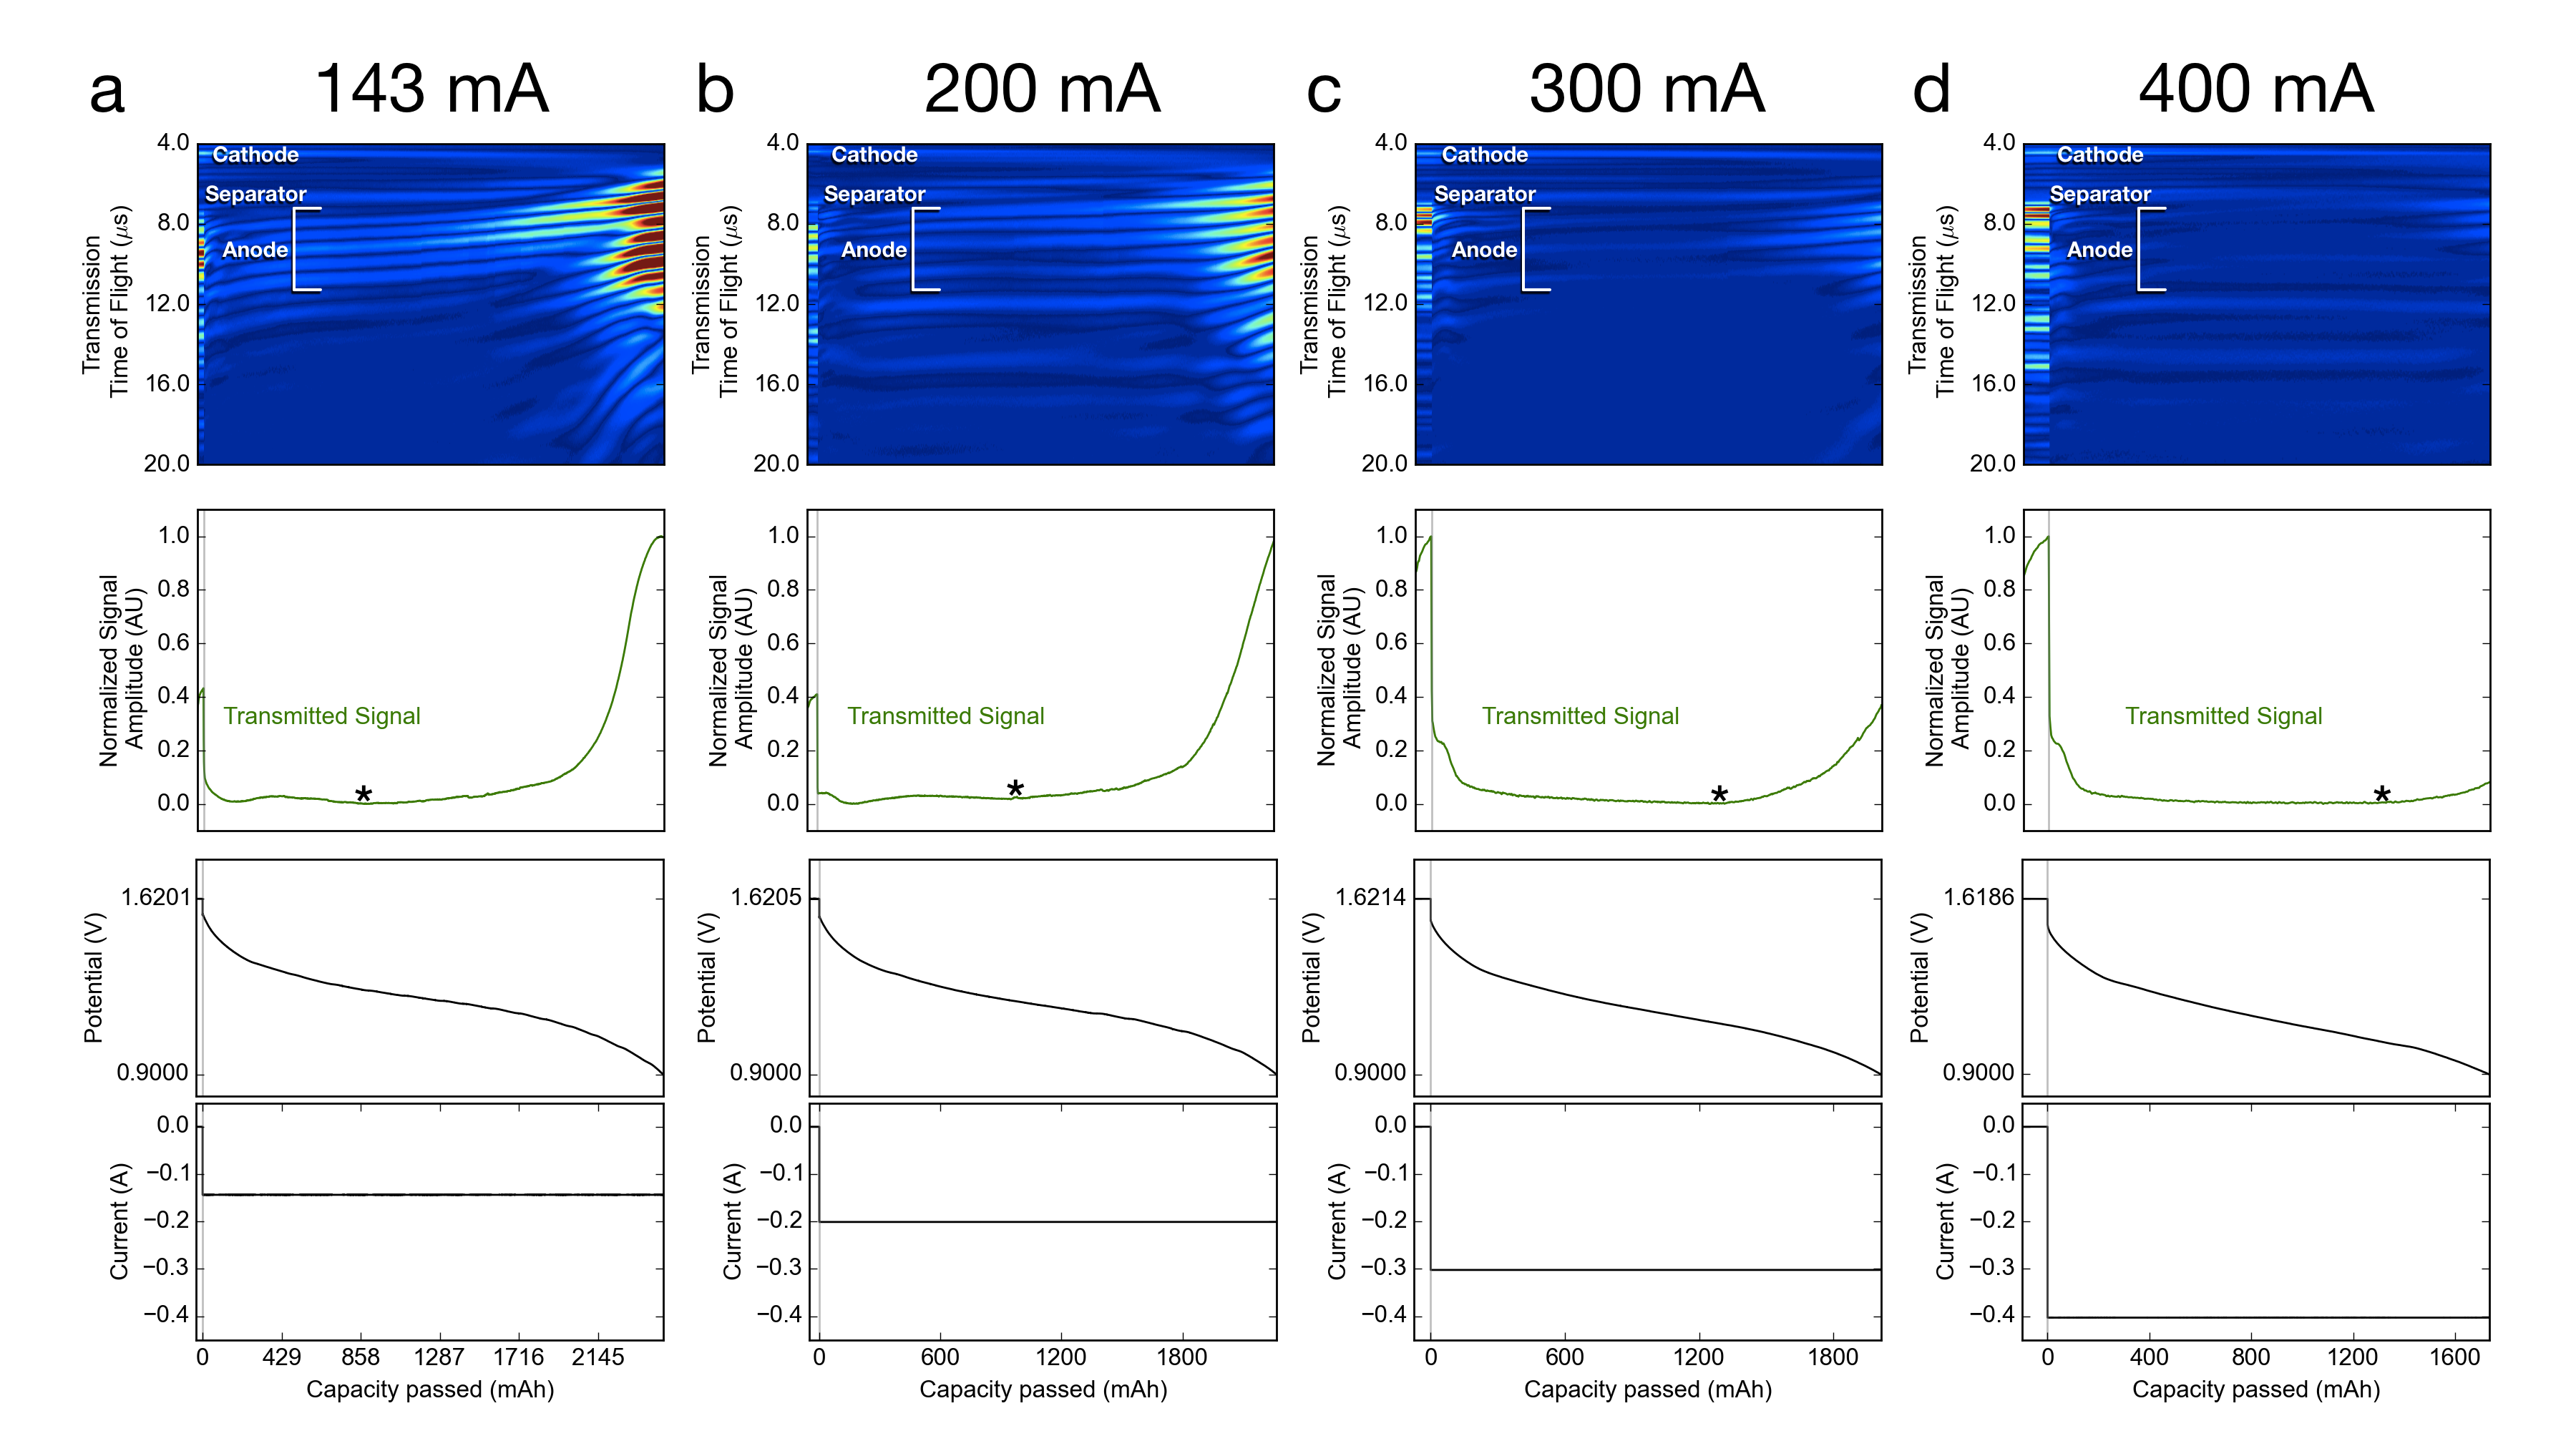
\includegraphics[width=1.00\textwidth]{ch5-alkbw/images/Fig1_v2.png}
    \caption[EAToF results for alkaline AA cells discharged at multiple rates.]{EAToF signal intensity maps, normalized total transmitted signal amplitude, potential, and current profiles for cells discharged at (a) 143 mA, (b) 200 mA, (c) 300 mA, (d) 400 mA. The estimated peak location/physical position correlations and the onset of increase in total transmitted signal amplitude are marked for each cell.}
    \label{fig:alkbwrates}
\end{figure}

In the transmission ToF maps for each cell, we observed a shift in peak position towards lower ToF as a function of depth of discharge, implying either an increase in modulus, or a decrease in density. As each cell approaches full discharge, we also observe an increase in the transmitted signal intensity, coupled with the appearance of peaks that were spaced evenly 0.7 $\pm$ 0.1 $\upmu$s apart. We posit that these evenly spaced peaks are indicative of an ``echo chamber," in which the ultrasonic pulse is reflected at either side until it constructively interferes in such a way that the pulse can transmit through to the receiver. The ToF maps all show a peak at 4.4 $\pm$ 0.1 $\upmu$s that does not shift like the higher order peaks, but does attenuate (i.e., decrease in intensity) more at lower discharge rates. We attribute this to the \ce{MnO2} cathode, which does not undergo appreciable density or modulus shifts,~\cite{Tao2013-vg} but does experience an influx of electrolyte during discharge, as shown by Riley et al through neutron tomography,~\cite{Riley2010-ur} particularly at lower discharge rates. As aqueous solutions attenuate acoustic signal more strongly than solids, it is expected that cells discharged at lower rates would experience greater attenuation of the peak we attribute to the~\ce{MnO2} cathode. In each cell, a ToF peak appears at 6.7 $\pm$ 0.05 $\upmu$s; in the 143 mA and 200 mA discharge cases this peak shifts to 6.4 $\upmu$s while increasing in signal intensity, however that same peak does not show any appreciable shifting and minimal intensification in the 300 mA and 400 mA discharge cases. We believe this ToF peak corresponds to the anode/separator interface, which is the site of the majority of ZnO formation at higher discharge rates (300 mA, 400 mA), hence the lack of higher order ToF echoes at end of discharge compared to the lower discharge rates (143 mA, 200 mA), as higher order ToF echoes would only appear in a mostly densified anode.

We also note that TTSA varies as a function of the discharge rate. The cell discharged at 143 mA shows an exponential increase in TTSA beginning around 900 mAh of capacity passed and continuing until the end of discharge at 2500 mAh of capacity passed. Similarly, the cell discharged at 200 mA shows an exponential increase in TTSA beginning at 969 mAh of capacity passed continuing until the end of discharge at 2264 mAh of capacity passed. In the cells discharged at 300 mA and 400 mA, there is noticeably less transmitted signal at the end of discharge compared to the initial state, with increases in TTSA at 1300 mAh and 1432 mAh capacity passed, respectively. In both, the TTSA at end of discharge is lower than TTSA at beginning of discharge. We expect such results, as the TTSA depends heavily on the oxidation of the anode from a signal-damping wet Zn gel into a more transmissive dry, porous ZnO solid. As previous work has shown,~\cite{Bhadra2015-aq,haibel,Manke2007-yj} the discharge rate will affect the overall distribution of ZnO within the anode of an alkaline bobbin-cell. Low discharge rates result in even and continuous formation of ZnO within the entire volume of the anode, whereas higher discharge rates result in rejection of electrolyte from the anode into the cathode and the subsequent formation of a ZnO crust at the anode/separator interface.~\cite{Riley2010-ur} The cells discharged at 100 mA and 200 mA would therefore show earlier densification of the entire volume of the Zn anode compared to the cells discharged at 300 mA and 400 mA, and the high discharge rate in the 300 and 400 mA cases may result in more expulsion of electrolyte into the anode/separator region, dampening the transmitted signal. We posit that the depths of discharge at which the TTSA begins to increase correspond to the point at which the anode has fully densified, meaning that the majority of the free volume of the anode consists of type I ZnO, as previously reported by Horn et al.~\cite{horn} The increase in TTSA of the 300 mA cell agrees well with previous work performed where coefficient of restitution was measured as a function of depth of discharge.~\cite{Bhadra2015-aq} At C/10 discharge rates, there was a saturation of coefficient of restitution  that occurred after roughly 1400 mAh of capacity were passed, corresponding to a densification of the anode. The exponential nature of the increase is likely due to the dehydration that occurs concurrently with oxidation in the anode, as the loss of residual moisture would result in less dampening of the transmitted pulse.

\subsection{EDXRD comparison}

To investigate these correlations more clearly, we compared the EAToF data to EDXRD data obtained in operando using beamline X17B1 at Brookhaven National Laboratory. Figure~\ref{fig:eatofedxrd} shows a portion of the time-resolved EDXRD map at the anode/separator interface and the ToF position of the transmission signal maximum during discharge. The range for the ToF peak position was chosen based on the understanding that the peak in all EAToF patterns at 7 $\upmu$s corresponds to the separator and that the maxima occurring at the end of discharge correspond to echoes from the central pulse based on the even separation in ToF of each maximum.~\cite{Trusler1991-ok} Portions of the EDXRD data are missing due to downtime of the synchrotron beam. Figure~\ref{fig:edxrdmap} provides a legend for interpreting peak positions in the EDXRD maps.

\begin{figure}[htb]
  \centering
    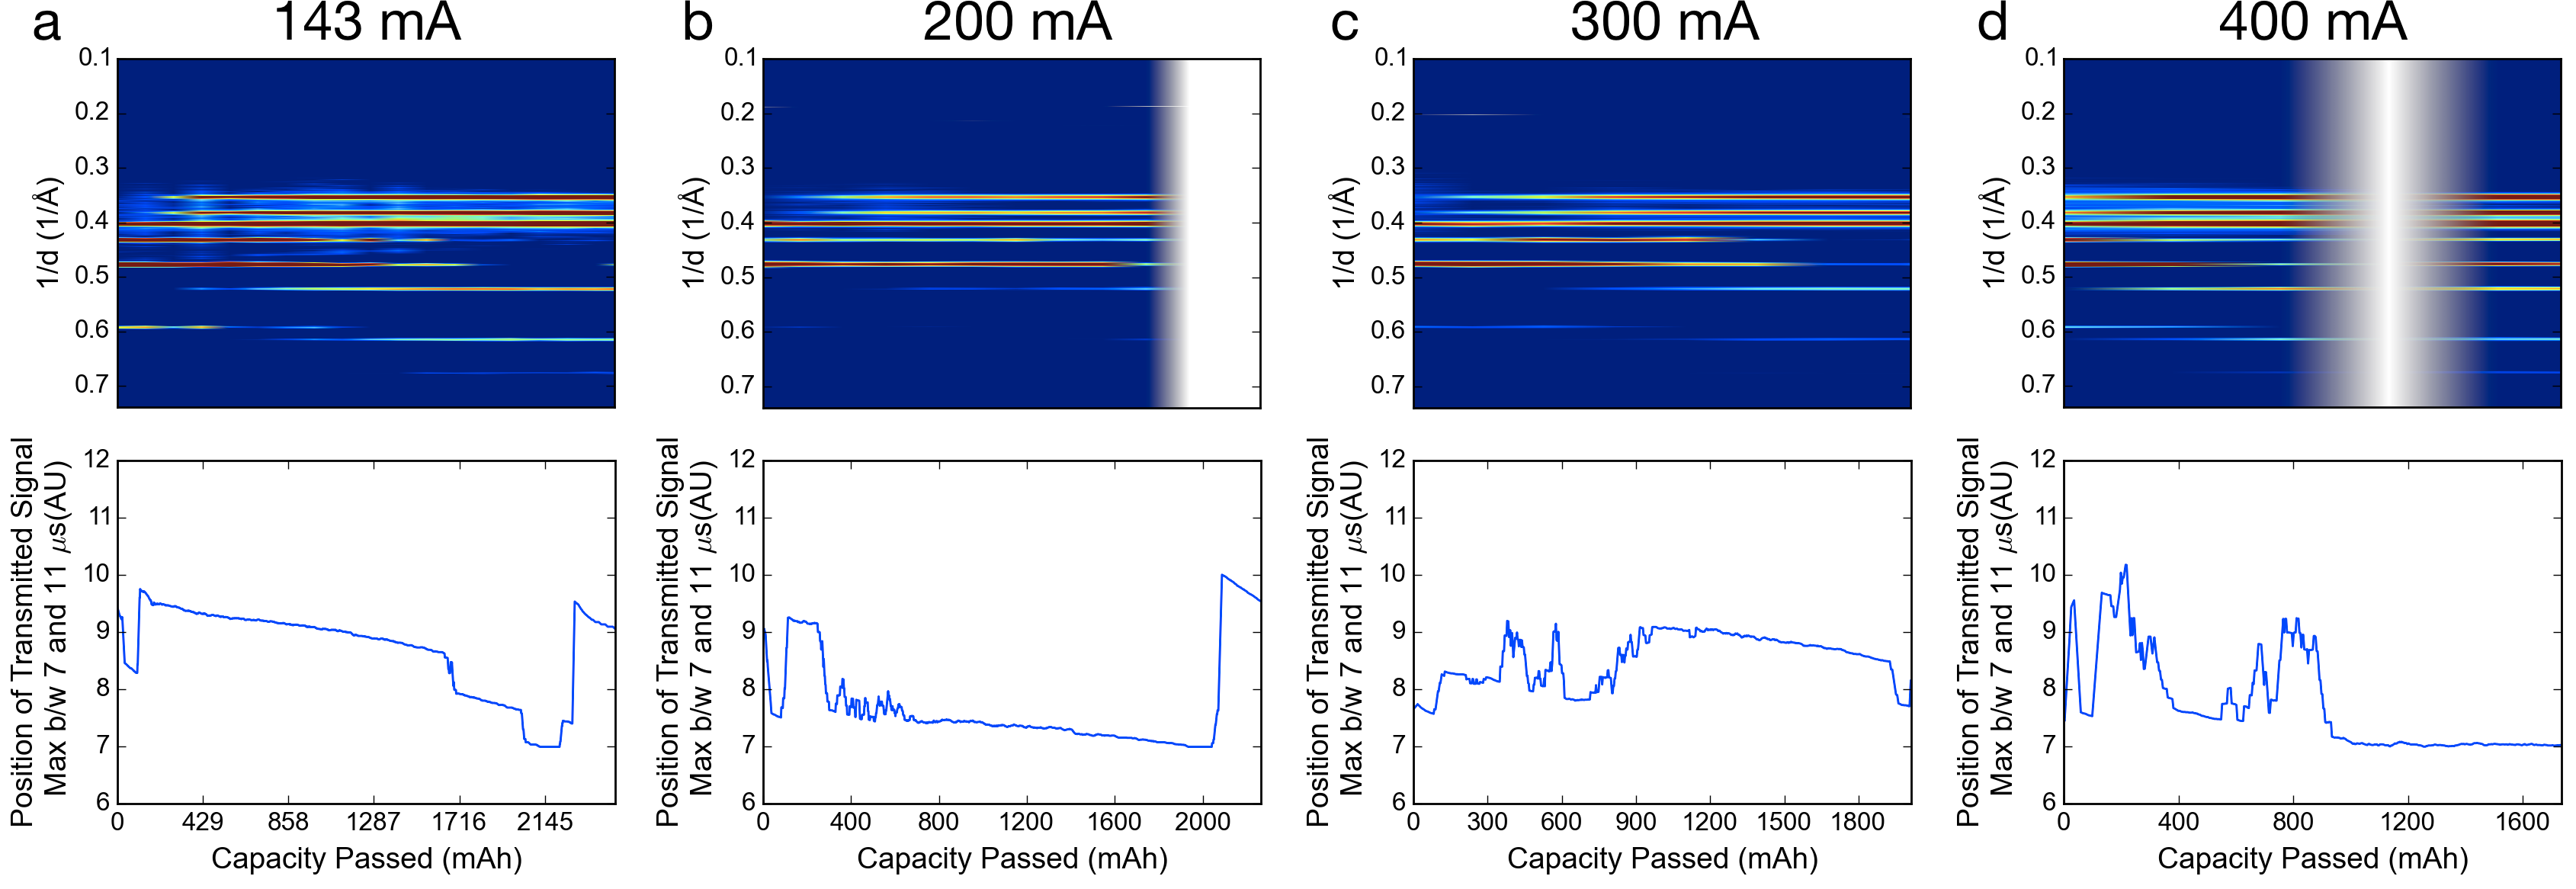
\includegraphics[width=1.00\textwidth]{ch5-alkbw/images/eatofedxrd.png}
    \caption[EDXRD maps of the anode/separator interface and transmitted EAToF max. position.]{Time-resolved EDXRD maps of the anode/separator interface and corresponding position of transmitted signal maximum between 7 and 11 $\upmu$s for cells discharged at (a) 143 mA, (b) 200 mA, (c) 300 mA, (d) 400 mA.}
    \label{fig:eatofedxrd}
\end{figure}

\begin{figure}[htb]
  \centering
    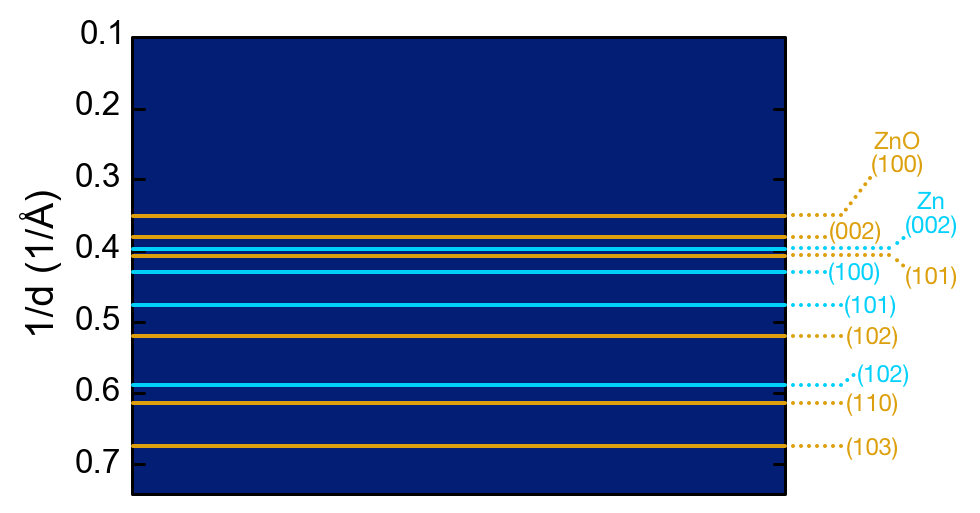
\includegraphics[width=0.8\textwidth]{ch5-alkbw/images/ZnPeakmap.png}
    \caption[Legend displaying peak positions in EDXRD maps.]{Legend displaying peak positions in EDXRD maps. Zn and ZnO peaks are labeled accordingly.}
    \label{fig:edxrdmap}
\end{figure}

Peak positions are given in the form 1/d(hkl). In all cells, we see a nearly instantaneous formation of ZnO as evidenced by the peaks at 0.356 \angstrom$^{-1}$(100), 0.385 \angstrom$^{-1}$(002), and 0.404 \angstrom$^{-1}$(101), with higher order peaks at 0.524 \angstrom$^{-1}$(102) and 0.616 \angstrom$^{-1}$(110) appearing later in discharge. Concurrently, we witness a weakening of some Zn peaks, specifically the 0.589 \angstrom$^{-1}$(102), 0.432 \angstrom$^{-1}$(100), and 0.476 \angstrom$^{-1}$(101) peaks. In the cell discharged at 143 mA the Zn(101) peak disappears entirely at 1955 mAh passed but reappears at 2414 mAh passed, implying possible redistribution of Zn near end of discharge. The ZnO(103) peak is only apparent in the cells discharged at 143 mA and 400 mA. This may correspond to a very dense region of the ZnO at the anode/separator interface, as at 143 mA, the entire anode densifies into a ZnO solid, while at 400 mA there is a very dense crust of ZnO that forms at the anode/separator interface.~\cite{haibel,horn,Bhadra2015-aq} The dense crust forms quickly after discharge begins, which explains the earlier appearance of the ZnO(103) peak in the 400 mA case (890 mAh passed) than in the 143 mA case (1430 mAh passed). This is further supported by the appearance of all measurable ZnO peaks in the scan range discharged at or near the beginning of discharge in the 400 mA case.

A number of correlations are visible between the EDXRD maps and the position of the ToF maximum for each cell. The cells discharged at 143, 200 and 300 mA all show an initial drop in ToF maximum, corresponding roughly to the appearance of the ZnO (100) and (002) peaks. All cells also show a negative slope in the position of the ToF maximum as a function discharge, with occasional jumps which we posit to be the formation of additional echo modes within the anode. This negative shift is expected during anode oxidation as the rigid, densified and dry ZnO allows for faster transmission of the ultrasonic pulse than the soft, wet Zn gel does. In the cell discharged at 143 mA we see a drop in ToF maximum from 8.69 to 8.03 $\upmu$s at 1650 mAh passed, which occurs 230 mAh after the appearance of the ZnO(103) peak and 300 mAh before the disappearance of the Zn(101) peak. The ToF continues to shift to lower values and drops from 7.71 to 7.16 $\upmu$s at 2050 mAh passed, 100 mAh after the disappearance of the Zn(101) peak and 40 mAh before the disappearance of the Zn(100) peak. The ToF maximum then jumps from 7.51 to 9.65 $\upmu$s at 2300 mAh passed, 114 mAh before the reappearance of the Zn(101). In the cell discharged at 200 mA we see a jump from 7.56 to 9.21 $\upmu$s at 80 mAh passed before a drop from 9.17 to 7.71 $\upmu$s at 255 mAh passed, which corresponds to a “hot spot” in the Zn(100) line. A period of fluctuation between 7.5 $\pm$ 0.2 and 8 $\pm$ 0.1 $\upmu$s follows between 277 mAh and 680 mAh passed, which corresponds to the disappearance and reappearance of the Zn(102) line. A monotonic decrease in ToF maximum then occurs until 2080 mAh passed, when there is a jump from 7.13 to 10.14 $\upmu$s. Unfortunately, this jump occurred during beam downtime, so we are unable to posit a reason based on the EDXRD data. In the cell discharged at 300 mA, the ToF maximum begins fluctuating between 8 $\pm$ 0.1 and 8.9 $\pm$ 0.2 $\upmu$s between 330 and 570 mAh passed. The beginning of this period of fluctuation corresponds to an intensification in the Zn(100) line, and the end corresponds to the appearance of the ZnO(102) line. Between 570 and 890 mAh passed the ToF maximum increases from 7.73 to 8.94 $\upmu$s, a difference of 1.21 $\upmu$s which is two times the minimum spacing between ToF echoes seen in the 143 and 200 mA cases. It has been shown previously that at 280 mA discharge rates, between 500 and 600 mAh passed there is a percolation pathway of ZnO-clad particles that forms from the separator to the central current collector in the Zn anode. Thus, we posit that the shift in ToF maximum is likely due to the formation of this percolation pathway. As the Zn(102) line decreases and the ZnO(110) line increases in intensity the ToF maximum follows a stable decrease from 8.94 to 8.3 $\upmu$s. The cell discharged at 400 mA showed the most fluctuation in ToF maximum. The appearance of the ZnO(103) line corresponds to the end of the first period of fluctuation between 110 and 380 mAh. As the Zn(101) line weakens around 550 mAh passed the ToF maximum begins fluctuating again, but appears to be in multiples of 0.7 $\pm$ 0.1 $\upmu$s, further supporting our “echo chamber” theory. From 932 mAh passed (roughly 55\% depth of discharge) to end of discharge the ToF maximum only shifts slightly from 7.12 to 6.91 $\upmu$s. The signal will not shift appreciably or intensify if there are no relevant density or modulus shifts occurring or if a path of least resistance for the transmitted pulse forms early. As the cell still provides another 800 mAh of energy, the latter case is likely what causes the stabilization of the ToF maximum as a dense ZnO crust forms at the anode/separator interface early into discharge and then continues to provide a path of least resistance for the transmitted pulse.

\section{Brand comparison}

Given the multitude of brands of alkaline AA batteries available to consumers, we wanted to determine the ability of EAToF to ascertain differences in the materials properties of multiple AA alkaline battery brands. To explore a range of batteries from most expensive to least expensive, we tested a combination of Duracell Quantum, Duracell Coppertop, CVS Alkaline, and Fujitsu G+ alkaline AA batteries. Cells were weighed as-received, then after cutting a 2 cm slit in the top of each cell. The cells were then desiccated for five days and weighed again. A sample of each battery’s Zn gel anode was also weighed as-received and again post-desiccation. As mentioned in Chapter~\ref{ch:pastwork}, alkaline AA batteries to weigh roughly 23.5 $\pm$ 0.5 g, but as shown in Table~\ref{tab:brandtable1}, the Quantum cell had a higher initial mass and a higher wet anode mass. This gives credence to Duracell's claims of a "Hi-Density Core" using "proprietary compression technology."\cite{duracell} The Quantum and Coppertop showed the same amount of moisture loss from the anode (within a margin of error), which was greater than that shown in the CVS and Fujitsu cells, implying improved hydration in the Quantum and Coppertop anodes. Furthermore, the Quantum and Coppertop showed an additional 0.3 g and 0.48 g of moisture loss from the entire cell, respectively, not including the 0.67 g of moisture lost from the anode, whereas the CVS and Fujitsu cells showed an additional 0.03 g and 0.02 g of additional moisture loss, respectively. This implies that the cathodes and separators in the Quantum and Coppertop cells are better hydrated. Better cell hydration would allow for greater electrolytic contact for all electrode components, and would manifest as a difference in capacity.

\begin{table}[htb]
\centering
  \caption[Alkaline AA battery mass and moisture loss by brand.]{\label{tab:brandtable1}Alkaline AA battery mass and moisture loss by brand. Margin of error in mass is $\pm$0.1 g.}
  \begin{tabular}[t]{*{5}{l}}
    \hline
       Brand & \specialcell{Cell mass (g)} & \specialcell{Total water\\content (g)} & \specialcell{Wet anode\\mass (g)} & \specialcell{Anode water\\content (g)}\\
    \hline
        Quantum   & 25.43 & 0.97 & 5.60 & 0.67\\
        Coppertop & 23.35 & 1.15 & 4.88 & 0.67\\
        CVS       & 23.21 & 0.46 & 4.71 & 0.43\\
        Fujitsu   & 23.72 & 0.62 & 4.88 & 0.60\\
  \end{tabular}
\end{table}

In addition to mass characterization, EAToF measurements were performed during discharge at 143 mA and 400 mA on all cells. A multiplexing circuit was used to run cells concurrently, which required additional amplification of the signal relative to the multiple discharge rate study. Cells were held at open circuit voltage for 15 minutes before discharge and discharged at constant current to a cutoff voltage of 0.9 V. Cells were then imaged using SEM \textit{post mortem} to visualize morphology changes that occurred during discharge. Table~\ref{tab:brandtable2} shows the relevant discharge capacities of each cell at 143 mA and 400 mA discharge rates. The Quantum cell displayed the closest to nameplate capacity (2850 mAh), with the Fujitsu cell showing the lowest capacity, showing a rough correlation of capacity with battery price. Furthermore, the Fujitsu cell performed very poorly at high discharge rates, showing only 25\% of nominal capacity at 400 mA. 

\begin{table}[htb]
\centering
  \caption{\label{tab:brandtable2}Alkaline AA battery discharge capacity by brand.}
  \begin{tabular}[t]{*{3}{l}}
    \hline
       Brand & \specialcell{Capacity at 143 mA\\(mAh)} & \specialcell{Capacity at 400 mA\\(mAh)}\\
    \hline
        Quantum   & 2456 & 1785\\
        Coppertop & 2311 & 1542\\
        CVS       & 2161 & 1452\\
        Fujitsu   & 2081 & 714\\
  \end{tabular}
\end{table}

\subsection{EAToF and SEM analysis of cells discharged at 143 mA}

Figure~\ref{fig:brand143} shows the time-resolved EAToF maps, the normalized TTSA, and the current and voltage profiles during discharge for each cell discharged at 143 mA. In the EAToF maps, it is clear that the Quantum AA shows a gradual increase in signal intensity over the full period of discharge, especially in the region determined to correspond to the anode. The Coppertop and CVS cells showed similar increases in signal intensity at the anode, but the CVS cell intensified slightly earlier and displayed a stronger shift to lower ToF values for higher order peaks. It is noted that the Coppertop cell displayed more echoes relative to the experiments performed in the previous section. We attribute this to the introduction of the multiplexing circuit, and the increased gain required to use that circuit. The Fujitsu cell showed strong anode transmission signal almost immediately. As we posited before, an intensification of the anode signal corresponds to the densification of the Zn gel anode into ZnO during discharge which implies that there may be more ZnO present initially in the Fujitsu cell due to possible self-discharge, which would contribute to the lower capacity relative to other brands. The Quantum cell shows only 6 evenly spaced echoes at end of discharge, compared to 7 for the Coppertop and 8 for the Fujitsu. We posit that this is due to differences in the capacities of each cell, such that the Quantum may still have appreciable capacity at 0.9 V, whereas the Fujitsu is completely “dead.” As a cell is used more, the anode becomes more dehydrated and more densely packed with stiff ZnO, thus counting the number of major echoes may provide a valuable metric in determining state of health in an alkaline cell.

\begin{figure}[htb]
  \centering
    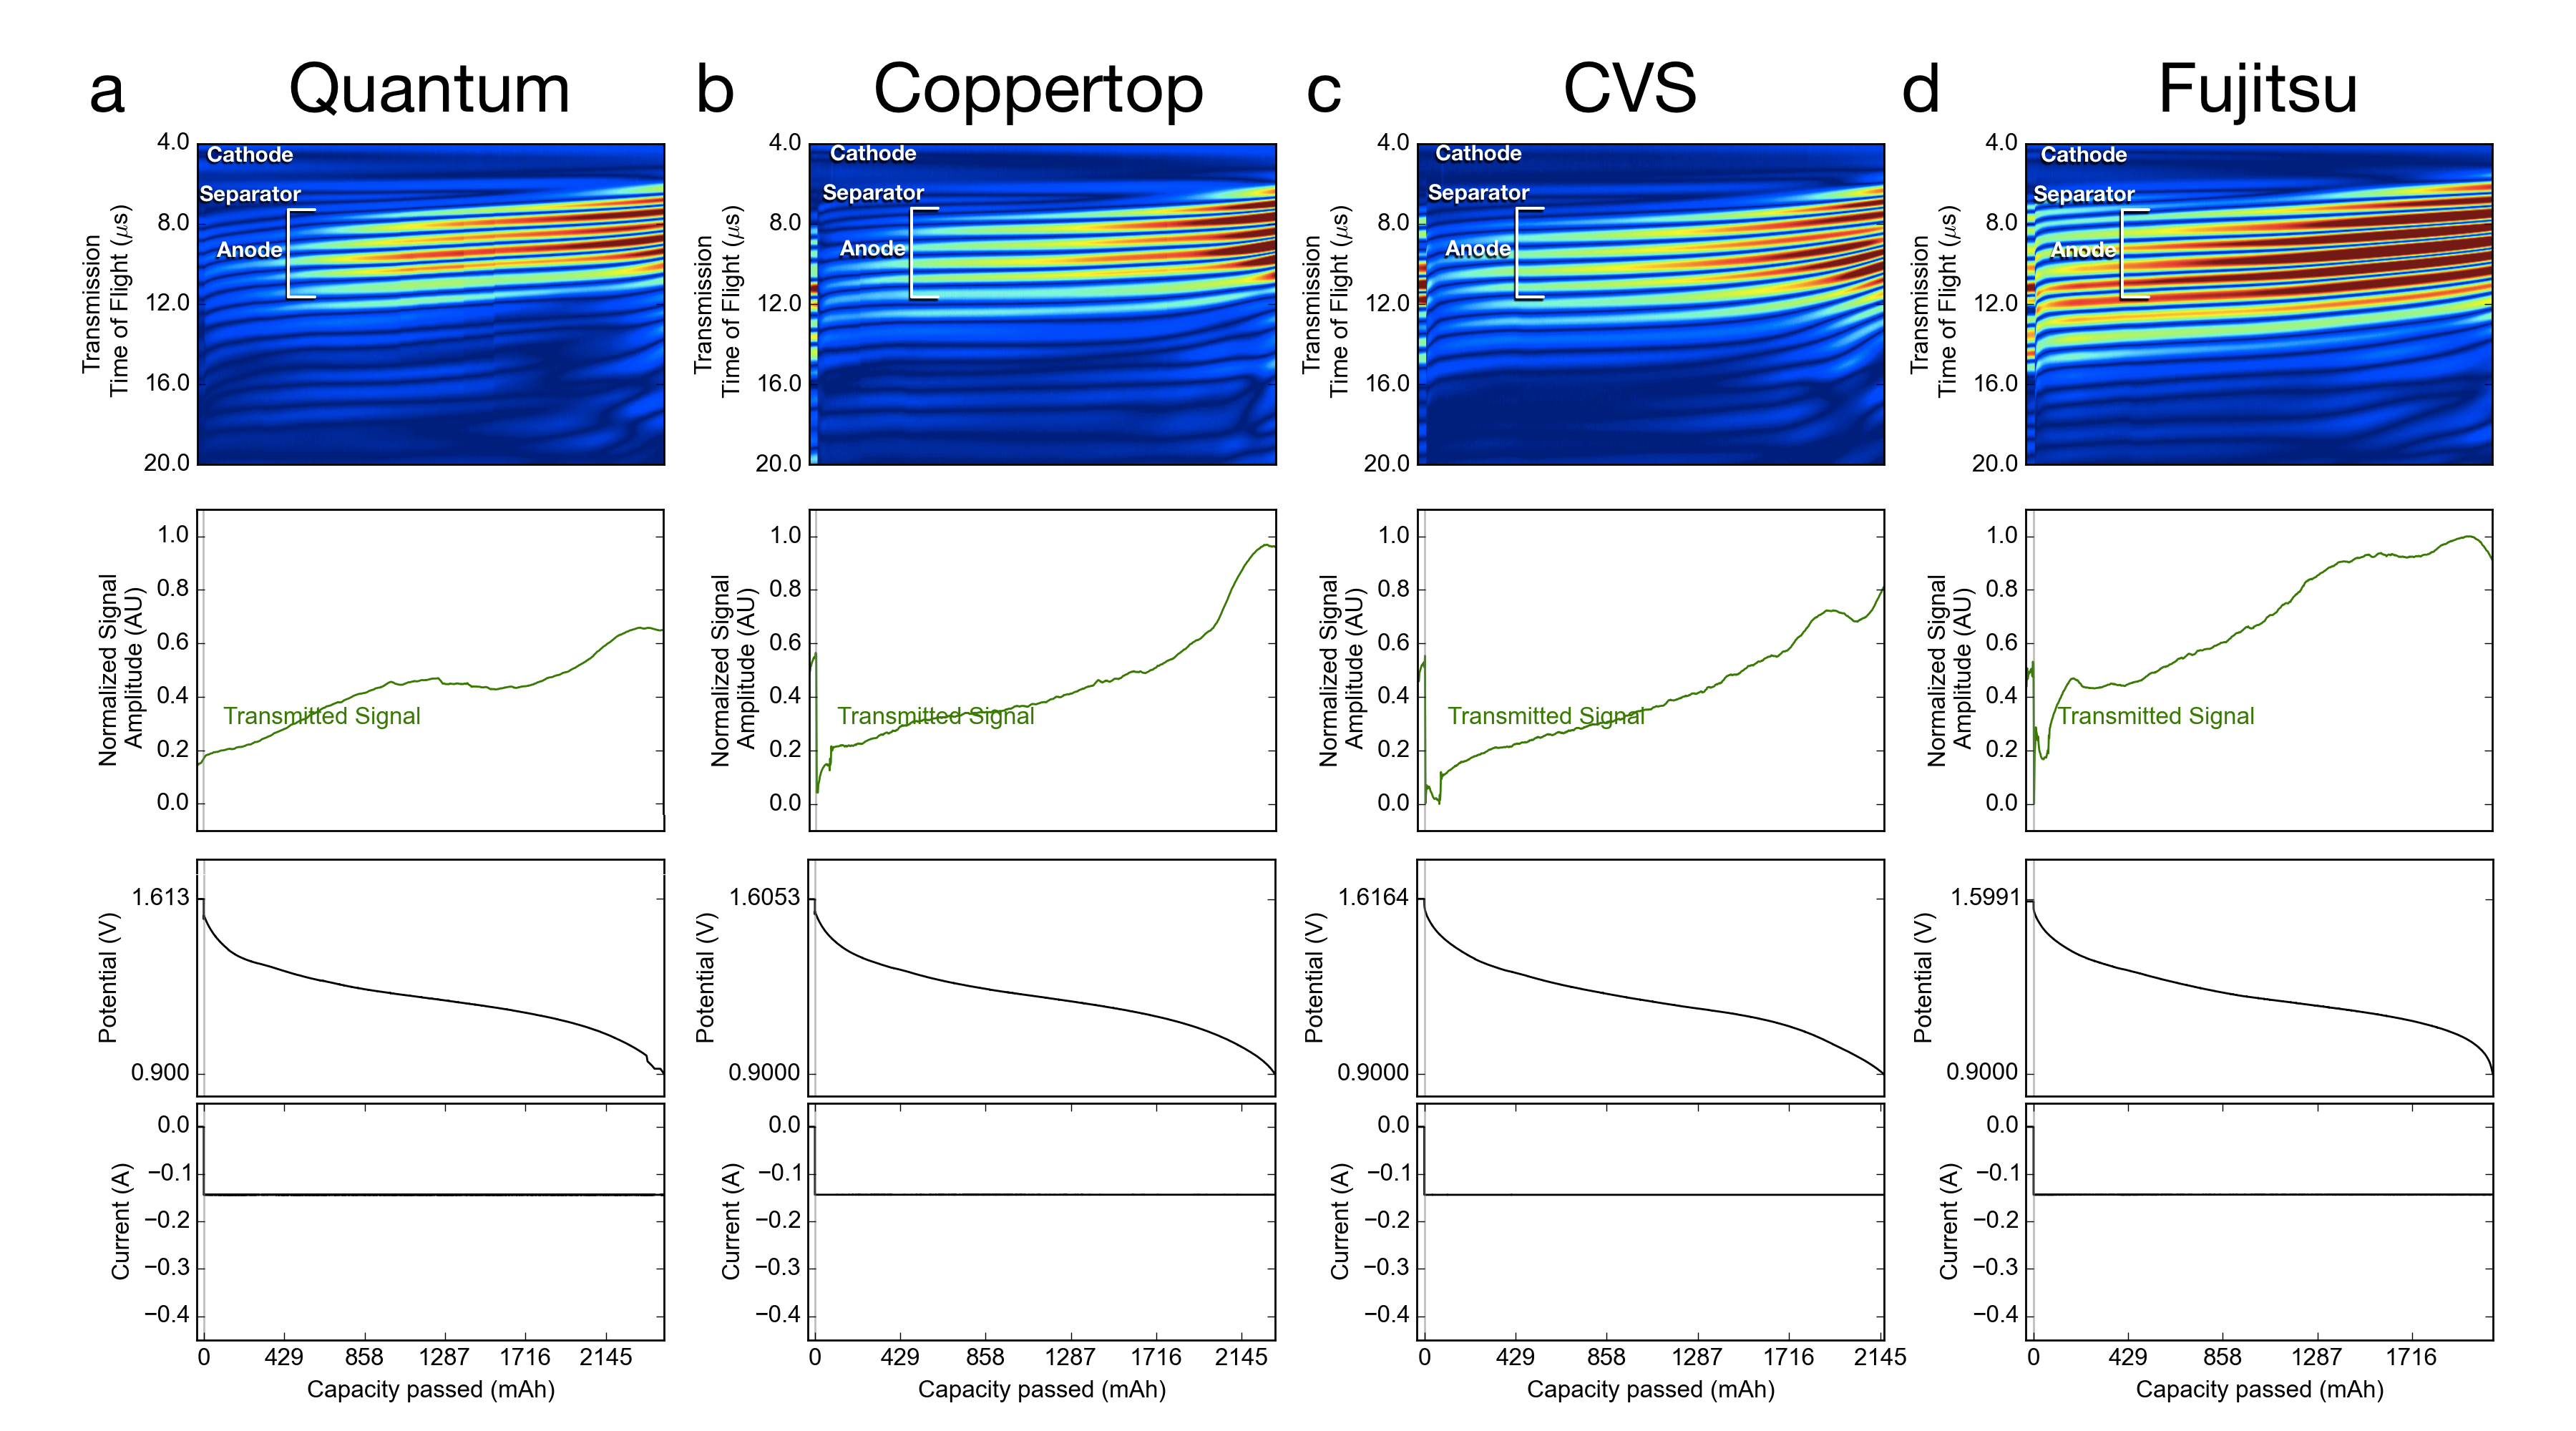
\includegraphics[width=\textwidth]{ch5-alkbw/images/BrandCompEAToF_143mA.png}
    \caption[EAToF results for multiple brands of alkaline AA cells discharged at 143 mA.]{EAToF signal intensity maps, normalized total transmitted signal amplitude, potential, and current profiles for (a) Quantum, (b) Coppertop, (c) CVS, and (d) Fujtisu cells discharged at 143 mA.}
    \label{fig:brand143}
\end{figure}

When observing the TTSA profiles for each, we note that the Quantum was the only cell not to display an initial drop in TTSA following rest, possibly caused by differences in transducer placement or pressure on the cell. The dip in TTSA at the onset of discharge may occur due to the dissolution of the surface layers of the discrete Zn particles that comprise the gel anode as they oxidize to \ce{Zn(OH)4^{2-}} ions in solution, creating a less connected pathway for the ultrasonic pulse to propagate.  Otherwise, all cells display an increase in TTSA during discharge, but with variations in the positions of local maxima and minima. In the Quantum, we see that a continuous increase in TTSA levels off and peaks around 1250 mAh passed, and then decreases slightly until 1550 mAh passed, at which point it again rises until 2350 mAh passed before leveling off again. The local minimum around 1550 mAh appears to correspond to a weakening of the near-separator EAToF peaks, which may be due to a local maximum in electrolyte rejection into the cathode, dampening the separator signal. This dampening would be negated once more ZnO forms in the anode. In the Coppertop, after the initial drop, the TTSA jumps quickly to 0.2 then gradually increases over the entire period of discharge until 2000 mAh passed, when the slope increases suddenly before leveling off at 2250 mAh. The sudden increase in slope may correspond to a combination of close to full dehydration and densification of the anode, as the removal of the electrolyte would result in an increase of signal transmitting through the ZnO solid. The reason this does not cause a local minimum as in the Quantum is likely due to its occurrence later in discharge when more of the anode has densified. The CVS cell displays similar TTSA behavior to the Coppertop, but experiences a minor increase in slope at 1700 mAh, a local maximum at 1900 mAh passed, and a local minimum at 2025 mAh passed. The increase in slope corresponds well to the point at which the higher order ToF peaks start shifting to lower ToF values, while the local minimum appears to correlate with a moment when some low order (~7 $\upmu$s) and higher order (>16 $\upmu$s) ToF peaks appear to weaken. A possible cause of this is destructive interference between the transmitted and reflected pulses within the anode. The Fujitsu cell displays a second initial dip in TTSA followed by a jump, which we believe to indicate the initial dissolution (dip) and precipitation of \ce{Zn(OH)4^{2-}} ions as solid ZnO. The point of precipitation depends heavily on the electrolyte pH and possible additives, and it is likely that in a less expensive cell there is less engineering that goes into inhibiting ZnO deposition via the chemistry of the electrolyte.

The \textit{post mortem} SEM analysis, shown in Fig.~\ref{fig:143sem}, shows that there were noticeable morphological differences between the cells. The Quantum cell shows a very uniformly densified anode, whereas the Coppertop shows a distinct region of densified anode and a region of discrete but connected particles. The CVS cell shows a very low level of porosity relative to the other cells, though the surface features lead us to believe that the lack of porosity may be due to crystallized KOH crystals that have filled the pores. This highly dense structure offers an explanation for the shift to lower ToF values at the end of discharge. The Fujitsu cell shows a very disjoint anode relative to the other cells, with discrete particles visible through the entire radius of the anode, which may explain the higher ToF values of the initial anode peaks, as a less connected ZnO pathway would result in longer transit times for the ultrasonic pulse.

\figskip{fig:143sem}

\begin{figure}[htb]
  \centering
    \includegraphics[width=0.8\textwidth]{ch5-alkbw/images/143_SEM.png}
    \caption[SEM micrographs of multiple brands of alkaline AA anodes after discharge at 143 mA.]{SEM micrographs of sectioned (a) Quantum, (b) Coppertop, (c) CVS, and (d) Fujtisu cell anodes discharged at 143 mA. Brass current collector is in the bottom-left of each image. Scale bar = 1 mm.}
    \label{fig:143sem}
\end{figure}

\clearpage

\subsection{EAToF and SEM analysis of cells discharged at 400 mA}

To further analyze how the cells performed under higher discharge rates, all brands were tested at 400 mAh. Figure~\ref{fig:brand400} shows the corresponding EAToF map, TTSA, and potential/current profile during discharge for each cell. This time, we see that the EAToF map for all cells shows an initial increase in intensity at the beginning of discharge, then some period of attenuation, followed by a final increase as the cell approaches the end of discharge. The Quantum cell displays strong signal intensity almost continuously. The Coppertop shows a similarly spaced peak profile to the Quantum with much weaker signal in the middle of discharge. The CVS and Fujitsu cells both show a more widely spaced peak profile with the end of discharge echoes clustered between 6 $\upmu$s and 12 $\upmu$s in the CVS cell, and a large number of low intensity echoes in the Fujitsu, the strongest clustered about 11 $\upmu$s, unlike the clustering of echoes between 8 $\upmu$s and 9 $\upmu$s in the other cells. 

\begin{figure}[htb]
  \centering
    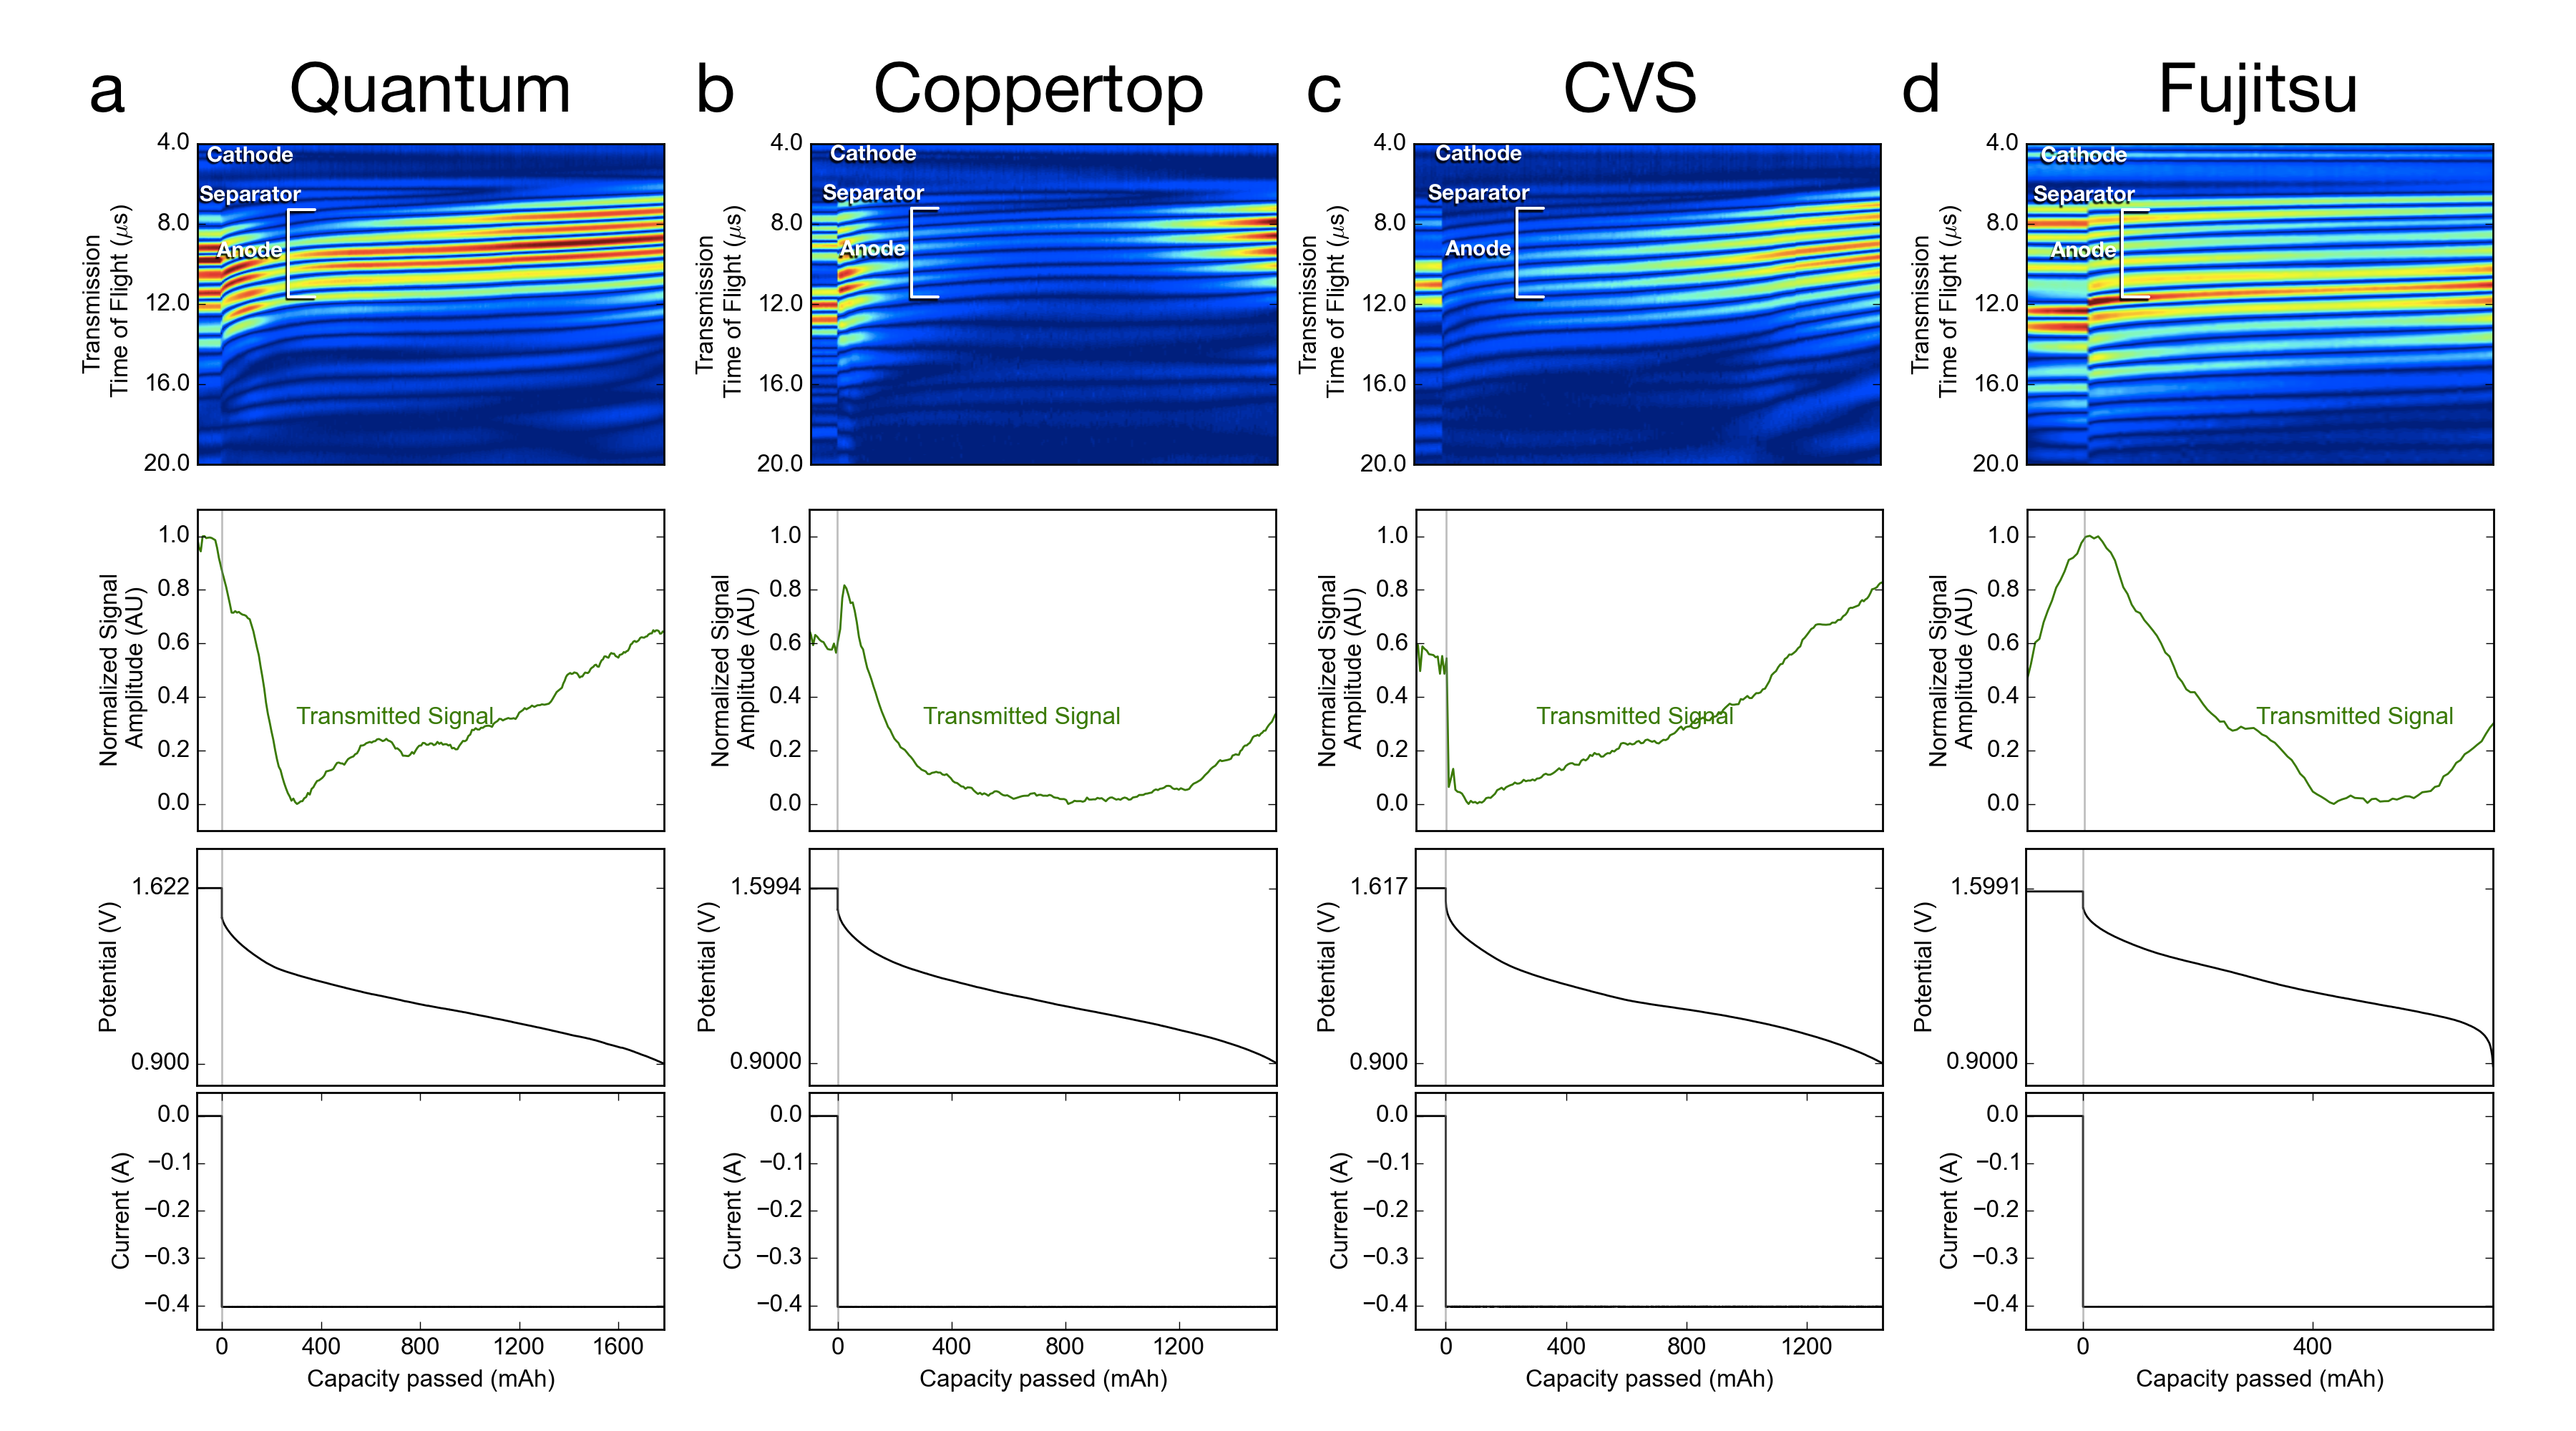
\includegraphics[width=\textwidth]{ch5-alkbw/images/BrandCompEAToF_400mA.png}
    \caption[EAToF results for multiple brands of alkaline AA cells discharged at 400 mA.]{EAToF signal intensity maps, normalized total transmitted signal amplitude, potential, and current profiles for (a) Quantum, (b) Coppertop, (c) CVS, and (d) Fujtisu cells discharged at 400 mA.}
    \label{fig:brand400}
\end{figure}

Looking at the TTSA profiles, we see that all cells display some degree of an initial decrease followed by an increase, though period of each varies largely from cell to cell. The initial increase in TTSA can be explained through the understanding that at high discharge rates, the anode will form a dense ZnO crust near the separator very soon after discharge begins. The decrease may correspond to the rejection of electrolyte from the center of the cell to the cathode, a process that would require the electrolyte to pass through the ZnO crust, decreasing the TTSA.  In the Quantum, we see an initially strong signal which decays over 315 mAh passed, then increases semi-monotonically until the end of discharge. In the Coppertop, we see an initial spike followed by a slow decay until 825 mAh passed, then a slow increase until end of discharge. The spike is higher than the TTSA during rest so it is possible that there is more initial densification, which would result in a slower transit of electrolyte across the densified ZnO crust and thus the long decay then increase in TTSA. The CVS cell shows a small initial spike in TTSA with a decrease until 100 mAh passed, and then increases monotonically. This would make sense if the ZnO crust does not form, but would be atypical for an alkaline AA cell. The Fujitsu cell displays a very peculiar increase in TTSA during rest, followed by a decay in signal over 255 mAh passed, then an increase until end of discharge at 714 mAh. This behavior is relatively similar to the first 800 mAh of discharge in the Quantum cell, implying similar rates of densification and electrolyte rejection. The rapid end of discharge in the Fujitsu cell could be a combination of oxidation limiting access to free surface in the anode and electrolyte starvation. 

\textit{Post mortem} SEM analysis, shown in Fig.~\ref{fig:400sem}, confirms a number of our assumptions from the EAToF measurements. The Quantum cell shows a much more thoroughly densified anode relative to the other cells, except the CVS cell. The CVS anode showed a largely smooth surface, which we attribute to the presence of residual KOH crystals, which we believe contribute to the low porosity. The Coppertop cell shows the characteristic ZnO crust near the separator at the upper right of the image, with a large area of discrete particles closer to the current collector at the lower left. The Fujitsu anode appears oxidized in a seemingly haphazard fashion, with some regions were densification has penetrated further into the anode, and others where there are discrete particles still visible near the separator.

\begin{figure}[htb]
  \centering
    \includegraphics[width=0.8\textwidth]{ch5-alkbw/images/400_SEM_correct.png}
    \caption[SEM micrographs of multiple brands of alkaline AA anodes after discharge at 143 mA.]{SEM micrographs of sectioned (a) Quantum, (b) Coppertop, (c) CVS, and (d) Fujtisu cell anodes discharged at 400 mA. Brass current collector is in the bottom-left of each image. Scale bar = 1 mm.}
    \label{fig:400sem}
\end{figure}

\subsection{Analysis of ToF shifts}

As in the discharge rate study, we also tracked peak position between 7 $\upmu$s and 11 $\upmu$s during discharge for all brands to determine how ToF evolution varied from cell to cell. The results are shown in Fig.~\ref{fig:brandpeak}.

\begin{figure}[htb]
  \centering
    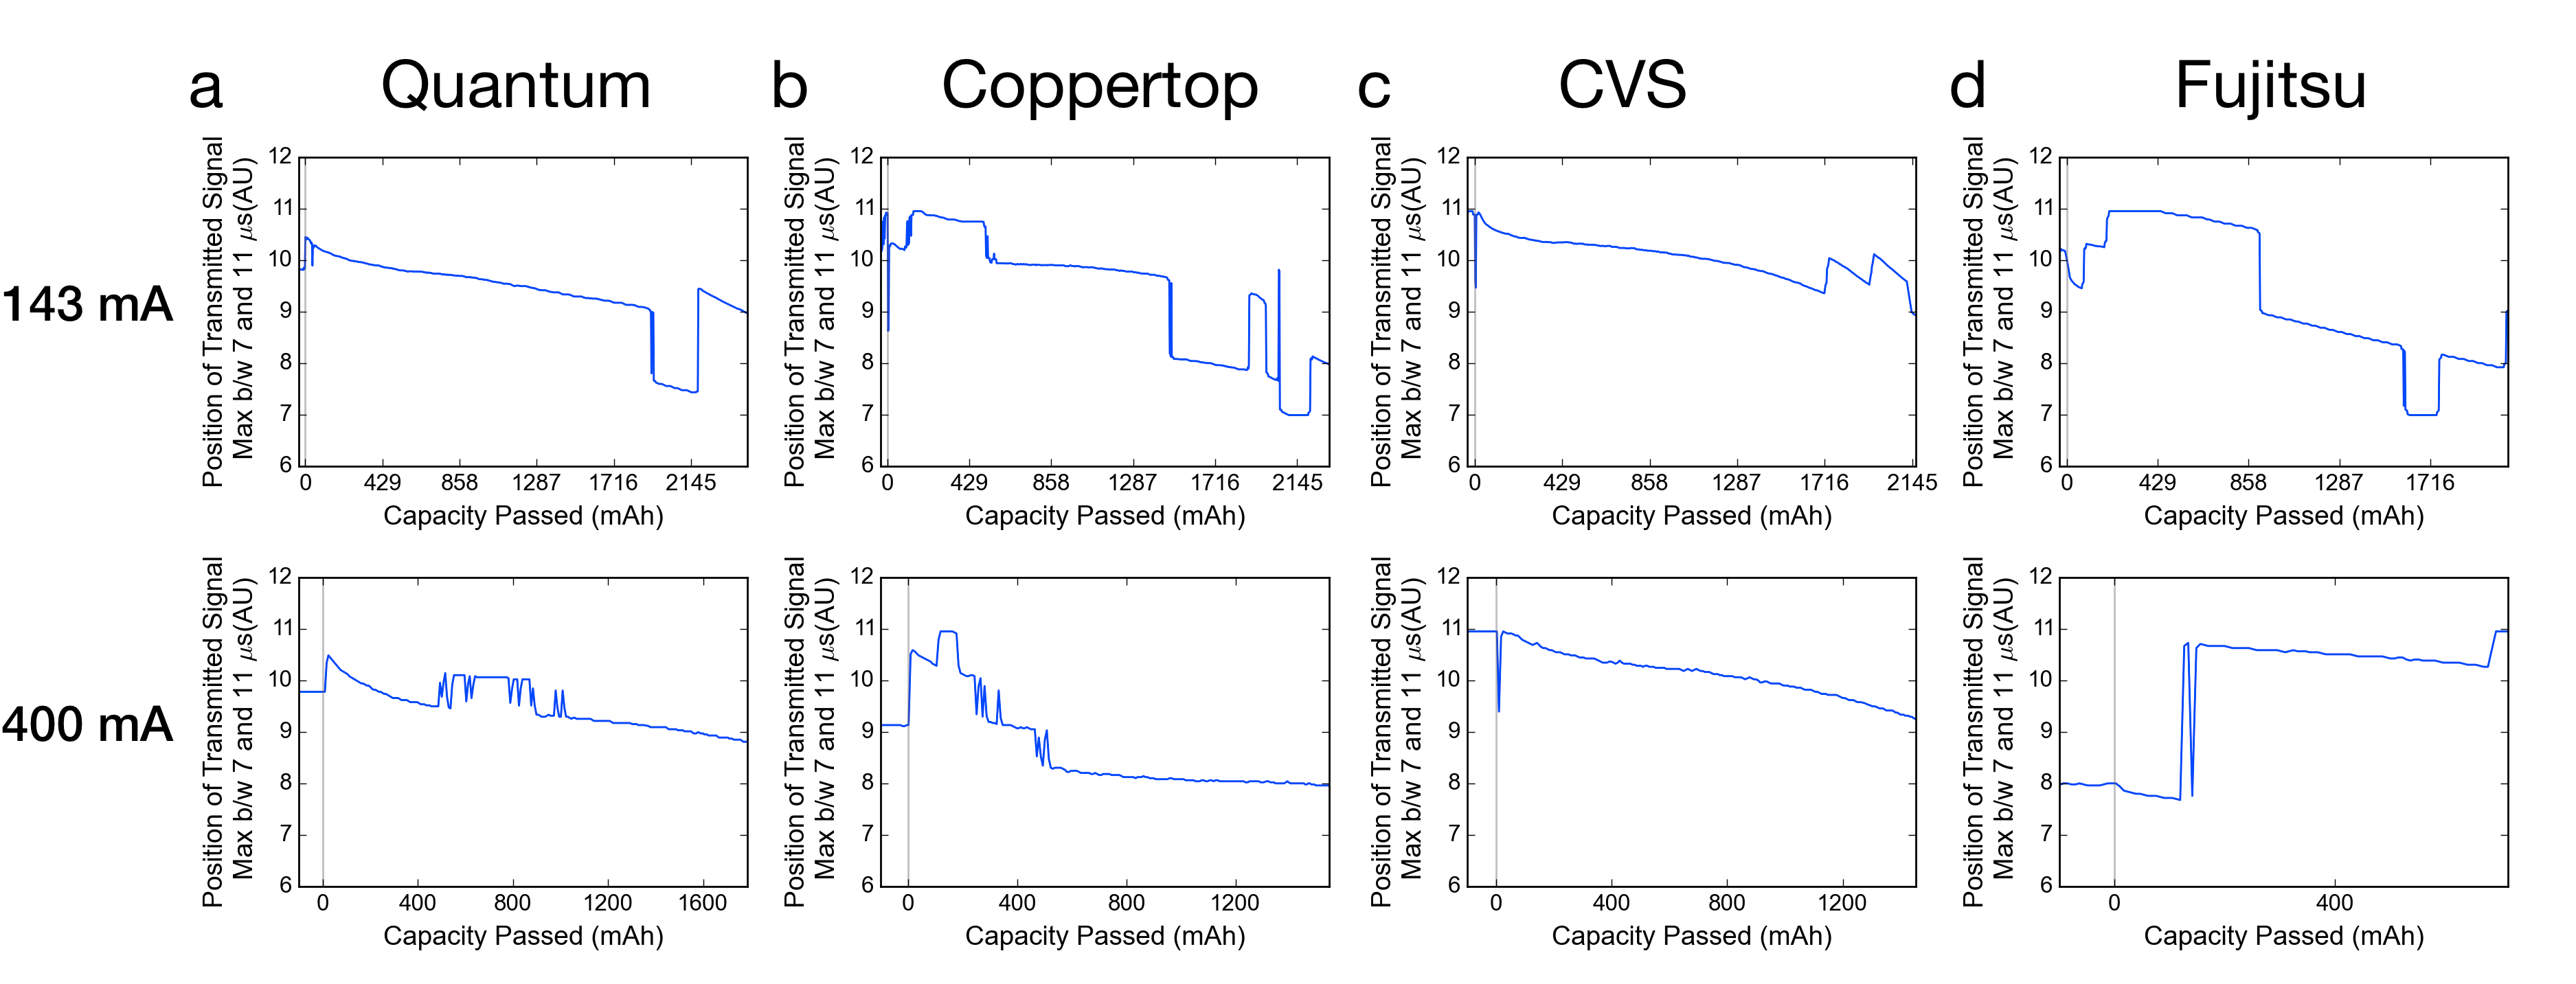
\includegraphics[width=\textwidth]{ch5-alkbw/images/BrandCompEAToF_PeakPos.png}
    \caption[ToF peak shifts for multiple brands of alkaline AA batteries.]{ToF peak shifts for multiple brands of alkaline AA batteries discharged at \textbf{top)} 143 mA and \textbf{bottom)} 400 mA.}
    \label{fig:brandpeak}
\end{figure}

In a number of cells, we noticed a Nernstian-like shift in the ToF positions, similar to shifts in the cell potential with discharge. In both the 143 mA and 400 mA discharge cases, the Quantum cell showed a jump from 9.8 $\upmu$s to 10.4 $\upmu$s. They also showed similar endpoints at roughly 8.9 $\upmu$s. The cell discharged at 400 mA showed a faster decrease in ToF position, as to be expected given the earlier oxidation that would occur from a higher discharge current. The period of fluctuation from 475 mAh to 1020 mAh was between 9.3 $\upmu$s and 10.0 $\upmu$s, again supporting our finding that echoes within the anode were spaced 0.7 $\pm$ 0.1 $\upmu$s apart. The Coppertop showed fluctuation at both discharge rates. At 143 mA the cell showed smaller (0.75 $\upmu$s) fluctuations, but later in discharge (1500 mAh passed) showed greater fluctuations (1.5 $\upmu$s to 2.1 $\upmu$s) which we attribute to increased oxidation and dehydration of the anode, leading to the creation of more echo modes. At 400 mA the fluctuations (0.6 $\upmu$s to 0.8 $\upmu$s) occurred between 0 mAh and 525 mAh before leveling off, which is expected as at the higher discharge rate, the bulk of the densification occurs early in discharge. The CVS cells both showed almost no fluctuation, with the 143 mA cell showing small fluctuations (0.6 $\upmu$s) at the end of discharge, and the 400 mA cell showing a single large fluctuation (1.5 $\upmu$s) at the beginning of discharge. Based on the SEM micrographs presented in Fig. 7 and 9, we think this is likely due to the low porosity densification of the anode, as the KOH crystals may scatter echoes more than a Zn/ZnO structure would. The endpoints are again similar (9.1 $\pm$ 0.1 $\upmu$s). The Fujitsu cell shows some fluctuation on the order of 0.8 $\upmu$s and 1.6 $\upmu$s in the 143 mA case, but maintains a decreasing trend in ToF position when fluctuations are ignored. In the 400 mA case, there is one large fluctuation of 3.0 $\upmu$s after 155 mAh passed, after which the ToF settles at the higher value of 10.7 $\upmu$s and then decreases until it jumps 0.7 $\upmu$s after 715 mAh passed. Unlike the other cells, the endpoints were very different: 9.0 $\upmu$s for the 143 mA cell and 10.9 $\upmu$s for the 400 mA cell. Comparing to the SEM micrographs we see that in the 143 mA cell the fluctuations are likely due to the disjoint nature of the oxidized anode, as at different points of discharge there may be a variety of pathways available for the ultrasonic pulse to travel along, and in the 400 mA cell the large jump is likely due to starvation of electrolyte, as it appears that there are few if any well-connected densified pathways for the ultrasonic pulse to travel along. The differences in final ToF value may be a result of the vastly differing levels of densification.

\subsection{Anode particle size and morphology comparison}

To further quantify differences in the material components of the four alkaline AA battery brands tested in this study, we removed a portion of the Zn anode particles and performed ex situ SEM analysis to determine particle size distributions. The SEM image is shown in Fig.~\ref{fig:znpart} and the particle size statistics are shown in Table~\ref{tab:zntable}.

\begin{figure}[htb]
  \centering
    \includegraphics[width=0.8\textwidth]{ch5-alkbw/images/Zn.png}
    \caption[SEM micrographs of Zn anode particles from multiple brands of alkaline AA batteries.]{SEM micrographs of Zn anode particles from (a) Quantum, (b) Coppertop, (c) CVS, and (d) Fujtisu cell anodes. Scale bar = 250 $\upmu$m.}
    \label{fig:znpart}
\end{figure}

\begin{table}[htb]
\centering
  \caption{\label{tab:zntable}Anode Zn particle size statistics by battery brand.}
  \begin{tabular}[t]{*{5}{l}}
    \hline
       Brand & \specialcell{Minimum size\\($\upmu$m)} & \specialcell{Maximum size\\($\upmu$m)} & \specialcell{Average size\\($\upmu$m)} & \specialcell{Standard deviation\\($\upmu$m)}\\
    \hline
        Quantum & 57 & 320 & 166 & 90\\
        Coppertop & 270 & 944 & 562 & 134\\
        CVS & 138 & 385 & 282 & 72\\
        Fujitsu & 107 & 1588 & 523 & 324\\
  \end{tabular}
\end{table}

All Zn particles appeared to be formed via spray pyrolysis given the characteristic “dog bone” and “potato” shapes of the individual particles.~\cite{linden} However, the particle size distributions vary widely. In the representative sample imaged for each cell, the Quantum particles were the smallest, ranging from from 57 um to 320 um. The CVS particles showed similar size distributions, ranging from 138 um to 282 um, but with flatter, fatter particles that showed a lower aspect ratio. The Coppertop particles tended to be longer than the Quantum and CVS particles, but showed higher aspect ratios. The Fujitsu particles appeared to be of the lowest quality, with a large spread in particle size distribution and some very large particles. As smaller particles would allow for more dense packing, it is expected that the Quantum would show the highest capacity and a stronger initial signal as shown in the ToF maps in Figs.~\ref{fig:brand143} and~\ref{fig:brand400}. Furthermore, smaller particles also have a higher surface to volume ratio, allowing for greater discharge capacity. 

The morphologies of the Zn anode gels also varied from cell to cell. The two Duracell cells (Quantum and Coppertop) displayed a paste-like consistency of the anode gels, which flowed and sheared easily. Conversely, the CVS and Fujitsu anode gels were stiffer and gummier, resisting deformation relative to the Duracell cells. We posit that this difference comes from the difference in gelling agents used in the electrolyte of each cell. The Fujitsu cell, in particular, was the most putty-like, which would provide an additional explanation for the stronger transmitted signal earlier in discharge as shown in Figs.~\ref{fig:brand143} and~\ref{fig:brand400}.

\subsection{Separator comparison}

During cell deconstruction, it was noted that the separators varied in thickness and qualitative feel from brand to brand. As such, we desiccated a portion of each separator and measured the thickness, then performed SEM analysis (Fig.~\ref{fig:seps}) to determine the fiber size distributions. 

\begin{figure}[htb]
  \centering
    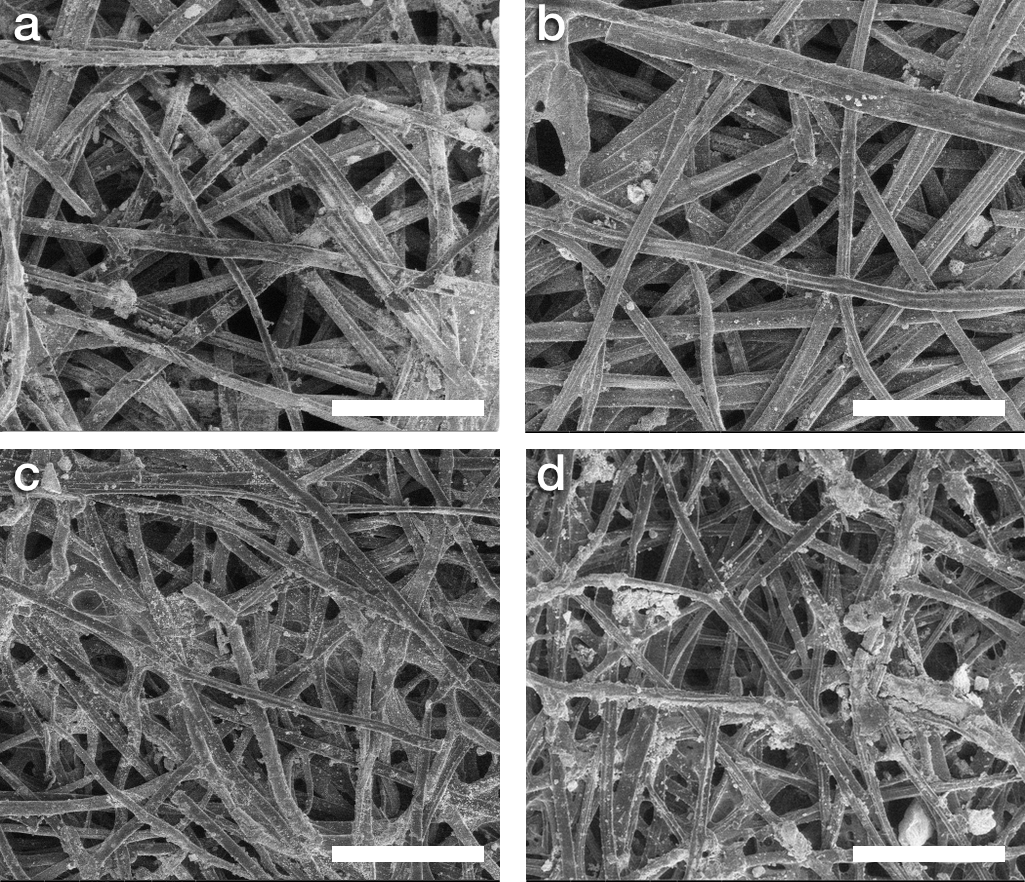
\includegraphics[width=0.8\textwidth]{ch5-alkbw/images/Seps.png}
    \caption[SEM micrographs of separators from multiple brands of alkaline AA batteries.]{SEM micrographs of separators from (a) Quantum, (b) Coppertop, (c) CVS, and (d) Fujtisu cells. Scale bar = 250 $\upmu$m.}
    \label{fig:seps}
\end{figure}

\begin{table}[htb]
\centering
  \caption{\label{tab:septable1}Separator fiber size statistics by battery brand.}
  \begin{tabular}[t]{*{5}{l}}
    \hline
       Brand & \specialcell{Minimum size\\($\upmu$m)} & \specialcell{Maximum size\\($\upmu$m)} & \specialcell{Average size\\($\upmu$m)} & \specialcell{Standard deviation\\($\upmu$m)}\\
    \hline
        Quantum   & 9.3 & 21.2 & 16.3 & 2.6\\
        Coppertop & 9.6 & 22.1 & 15.9 & 3.3\\
        CVS       & 8.3 & 15.0 & 11.3 & 1.6\\
        Fujitsu   & 7.8 & 13.5 & 10.6 & 1.6\\
  \end{tabular}
\end{table}

The SEM micrographs in Fig.~\ref{fig:seps} and the data in Table~\ref{tab:septable1} show that the Quantum and Coppertop separators were more robust at the microscale, with larger diameter fibers relative to the CVS and Fujitsu separators. It is of note that despite the increased fiber size, the Quantum and Coppertop separators had smoother textures than the CVS and Fujitsu separators. The two Duracell brand separators both had a smooth texture and were 80 um in thickness, while the CVS and Fujitsu separators appeared fibrous at 110 um and 120 um respectively, as detailed in Table~\ref{tab:septable2}.

\begin{table}[htb]
\centering
  \caption{\label{tab:septable2}Separator thickness and texture by battery brand.}
  \begin{tabular}[t]{*{3}{l}}
    \hline
       Brand & \specialcell{Thickness ($\upmu$m)} & Texture \\
    \hline
        Quantum   & 80  & smooth\\
        Coppertop & 80  & smooth\\
        CVS       & 110 & fibrous\\
        Fujitsu   & 120 & fibrous\\
  \end{tabular}
\end{table}

The construction of the separators varied from cell to cell. The Quantum contained two thin rectangular sleeves that were folded in half and rotated 90~\degree from each other as demonstrated in Fig.~\ref{fig:sepassembly}a,~\cite{Anglin2010-cj} while the CVS and Fujitsu cells had single-piece separator sleeves as demonstrated in Fig.~\ref{fig:sepassembly}b.~\cite{fujitsu} The Coppertop also contained a thin cellophane sleeve around the separator encased anode. The thickness of the separator could contribute to increased cell impedance, and hence the lower capacities of the CVS and Fujitsu cells. Beyond this conclusion, however, we are unable to draw any strong correlations to the EAToF measurements performed on these cells.

\begin{figure}[htb]
  \centering
    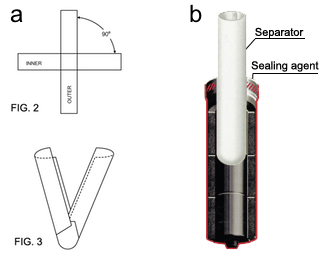
\includegraphics[width=0.7\textwidth]{ch5-alkbw/images/SepAssembly.png}
    \caption[Two separator configurations in alkaline AA batteries.]{Separator configurations for \textbf{a)} Quantum and Coppertop batteries and \textbf{b)} CVS and Fujitsu batteries.}
    \label{fig:sepassembly}
\end{figure}






